
This \stone idea originates in chapter 9.2 of \textcite{simp17}. 

We solve the full 2D surface evolution model 
\begin{equation}
\frac{\partial h}{\partial t}
+ u \frac{\partial h}{\partial x}
+ v \frac{\partial h}{\partial y}
= \vec\nabla\cdot \left[ (c_0 + c A_e^r S^{m-1}) \vec\nabla h \right] + w
\end{equation}
without lateral tectonic advection, that is,
\begin{equation}
\frac{\partial h}{\partial t}
= \vec\nabla\cdot \left[ (c_0 + c A_e^r S^{m-1}) \vec\nabla h \right] + w
\end{equation}
where $h$ is the surface elevation, 
$c_0$ is the ``hillslope'' diffusivity, 
$c$ is a fluvial transport coefficient, $A_e$ 
is the effective upstream drainage area (defined as $A_e = A - A_c$ 
where $A$ is the upstream drainage
area and $A_c$ is a critical drainage area below which there is no fluvial sediment transport),
$S$ is the slope, 
$r$ and $m$ are positive exponents, and $w$ is the rate of rock uplift (assumed to be uniform and constant).

This equation will be solved on a square $50\times 50~\si{\km}$ 
domain that has an initial random elevation of
between 0 and 10 m, while the elevation of all four boundaries is fixed to zero. 
Here, we use linear three-node triangular elements.

The finite element formulation of the equation above is 
\[
\M \cdot \vec{\dot h} + \K \cdot \vec{h} = \vec{F} 
\]
with 
\begin{eqnarray}
\M &=& \int_\Omega \vec{\bN}^T \vec{\bN} dV \; \nn\\
\K &=& \int_\Omega {\bm B}^T (c_0 + c A_e^r S^{m-1})  {\bm B} \;  dV \nn\\
\vec{F} &=& \int_\Omega  \vec{\bN}^T w \; dV
\end{eqnarray}
where $\vec{h}$ is the vector of nodal elevations for an element, $\vec{\bN}$ 
are the shape functions, ${\bm B}$ are the shape function derivatives expressed 
in terms of physical coordinates.

Using a first-order time derivative yields
\[
(\M  + \K \delta t ) \cdot \vec{h}^n = \vec{F}  + \K \cdot \vec{h}^{n-1}
\]
Except for the coefficient inside the $\K$ matrix, this is a rather standard diffusion equation. 
Looking closer, the upstream drainage area $A$ appearing in the element matrix $\K$ 
(recall that $A_e = A - A_c$ ) is computed according to the following scheme:
\begin{enumerate}
\item Calculate the surface area of each finite element. In the program listed in the following text, the
result is saved in the array {\tt area}.
\item Find and save the three elements adjacent to each element, 
saved in the array {\tt gnei}\todo{change name!}. 
Elements on the boundary that have only two neighbors are assigned their own element index to the missing
third neighbor. If the mesh doesn't change through time, this step and the previous one need to
be performed only once before the time loop.
\item  At each step in time, calculate the average elevation of each element, based on the three corner
nodes. The result is saved in the array {\tt zc}.
\item Sort the average element elevation for the entire mesh from highest to lowest. The indices of the
sorted elevations are saved in the array {\tt sorted\_indices}.
\item Using the sorted indices, sort the neighboring elements, the result of which is saved in
{\tt sorted\_gnei}. At this stage, all elements in the mesh have been ordered, along with their three
adjacent neighbors, from highest to lowest.
\item For each element, find and save the local index of the lowest of the three adjacent elements. The
result (i.e., 1, 2, or 3) is saved in the array {\tt min\_index}.
\item Set the upstream drainage area {\tt A} initially to the element area.
\item In a loop over all ordered elements from highest to lowest, ``pass'' the accumulated drainage area
from each (donor) element to its lowest adjacent neighbor (receiver). The result after the loop has
been completed is the accumulated surface area that ``drains'' to each element in the landscape, {\tt A}. 
Note that this procedure implicitly assumes a spatially uniform rainfall, which can easily be
accounted for if desired.

\end{enumerate}

\newpage
\begin{center}
\fbox{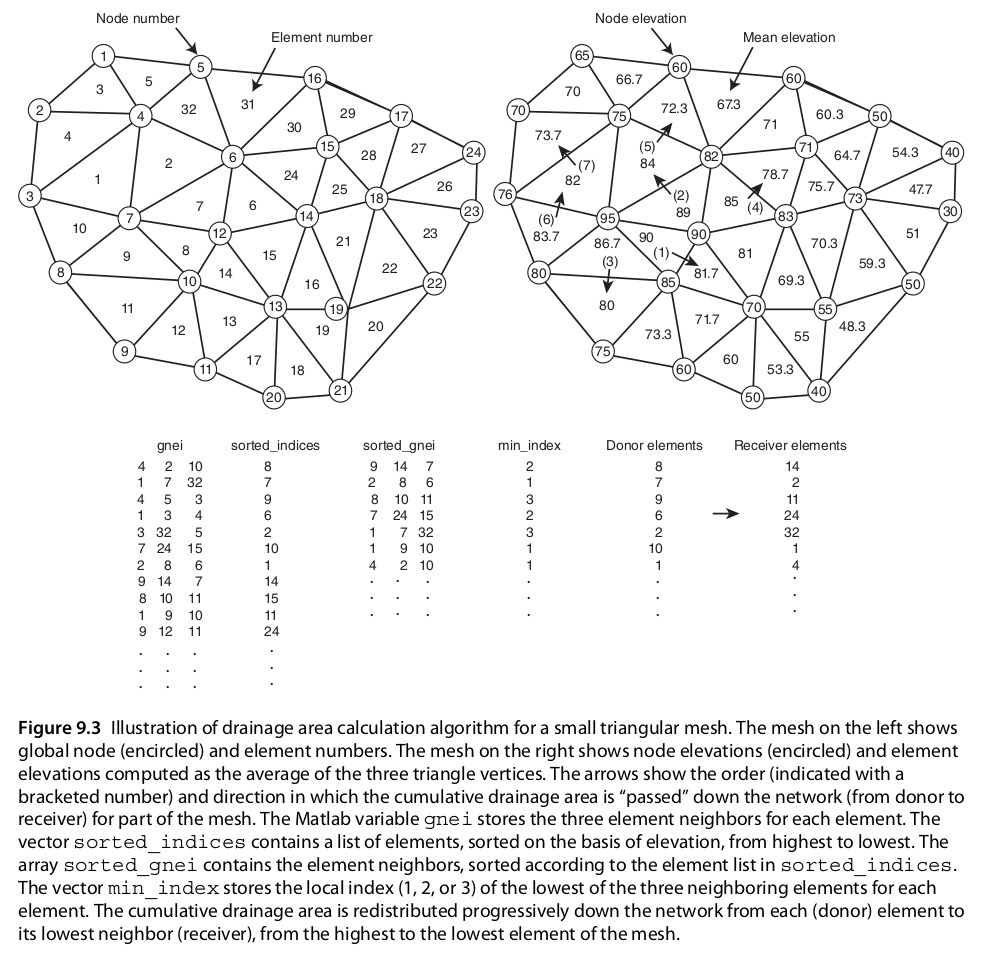
\includegraphics[width=12cm]{python_codes/fieldstone_140/images/simp1}}\\
\fbox{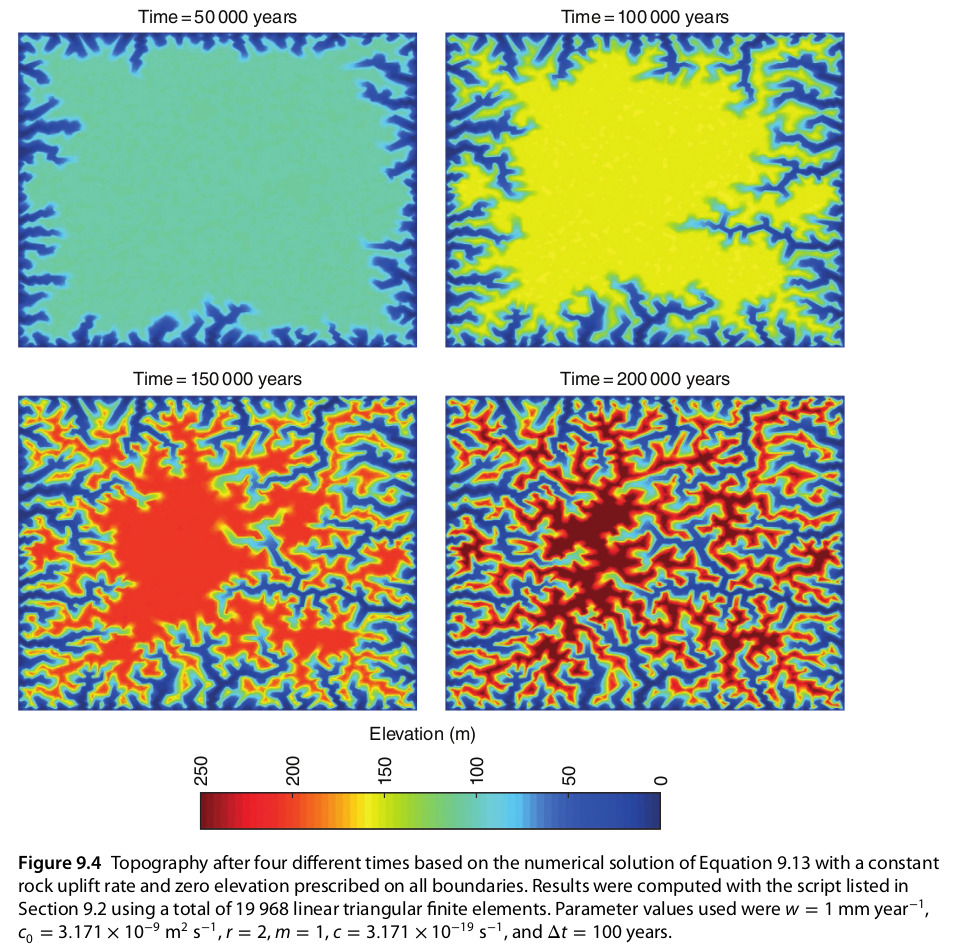
\includegraphics[width=12cm]{python_codes/fieldstone_140/images/simp2}}
\end{center}

Questions:
- his quadrature is weird?  3 pts see table 7.2???


